\section{Future Work}

\subsection{Domain Decomposition}

Right now our solver only works on a single continuous allocation
for the entire domain.
Allowing the domain to be split over many blocks would have several 
advantages.
\begin{itemize}
  \item \textit{Utilizing Additional Memory } \\
My Macbook has a limit on storage buffer sizes of a little over $4$gb.
Domain decomposition would allow me to utilize more buffers, and thus more of the $64$gb I have available.

  \item \textit{Distributed Computing} \\
Distributing the solve over several compute nodes would require 
domain decomposition. 
This could be multiple GPUs in one system or
multiple compute nodes in an HPC environment.

  \item \text{Spatial Adaptivity} \\
Most exciting, domain decomposition would be the next step towards spatial adaptivity, see Figure \ref{fig:adaptivity}. 
Spatial adaptivity would allow the limited memory resources to
capture a greater amount of detail in turbulent flows.
\end{itemize}
\begin{figure}
\label{fig:adaptivity}
\begin{center}
  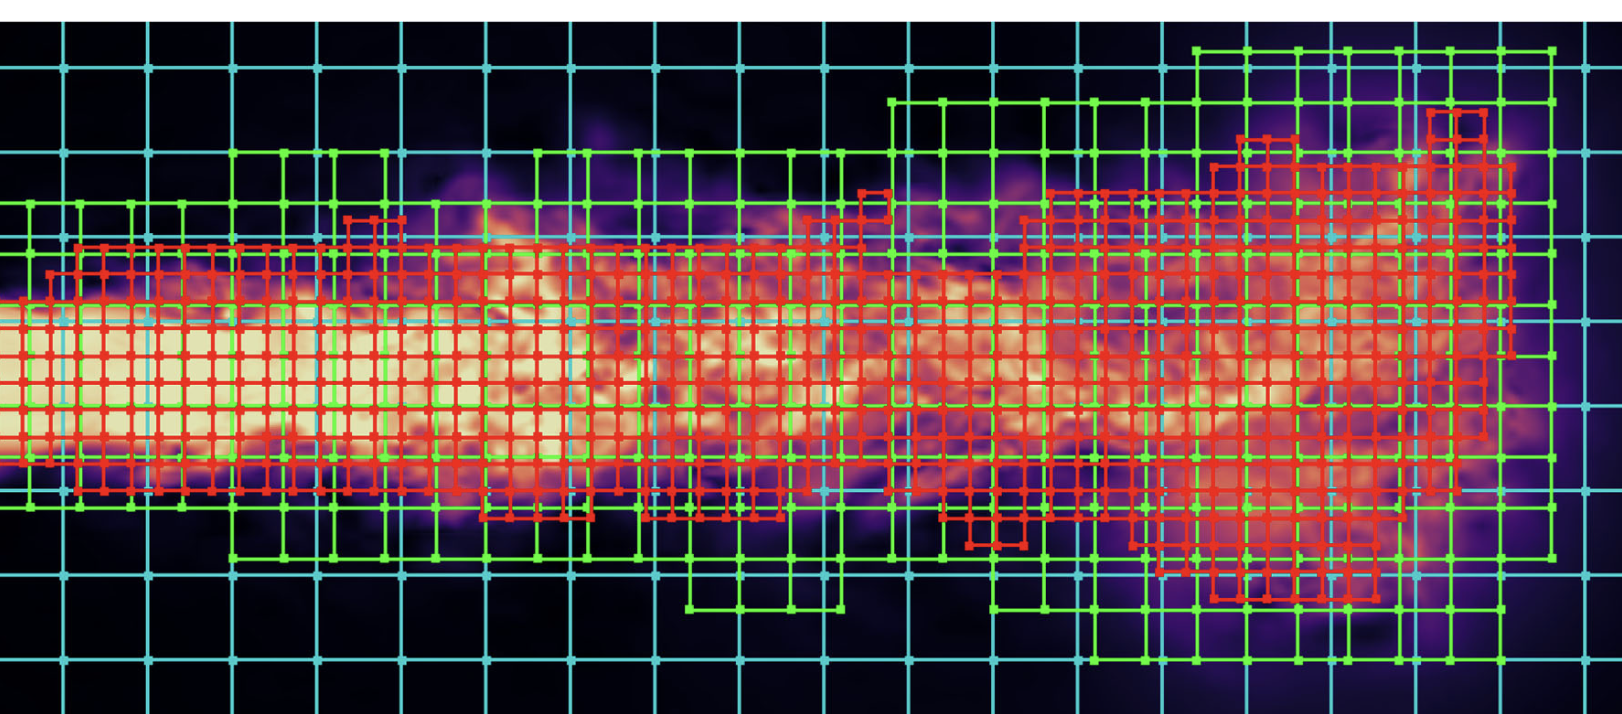
\includegraphics[width=0.6\linewidth]{adaptivity.png}
\end{center}
\caption{Spatial adaptivity allows the solver to resolve important features at higher resolutions. The above is from \cite{Li2018} which described an adaptivity scheme for CM-MRT}
\end{figure}
